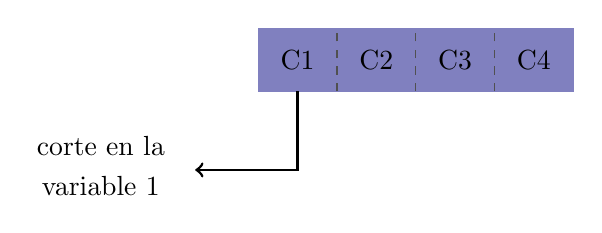
\begin{tikzpicture}[scale=1]
    \colorlet{c1}{blue!50!black!50}
    \colorlet{c2}{red!50!black!50}
    \colorlet{gray}{gray!40!black!80}

    \draw[c1, fill] (0,0.2) rectangle (4,1);

    \draw node at (0.5, 0.6) {C1};
    \draw node at (1.5, 0.6) {C2};
    \draw node at (2.5, 0.6) {C3};
    \draw node at (3.5, 0.6) {C4};

    \foreach \x in {1,2,3} \draw[dashed,gray] (\x,0.2) -- (\x,1);

    %% \draw[->,line width=2] (2,-0.5) -- (2,-2.3);

    %% \draw node at (2, -3) {\small "VAR1$>$C1 \&\& VAR2$>$C2 \&\& VAR3$>$C3 \&\& VAR4$<$C4"};

    \draw node at (-2,-0.5) {corte en la};
    \draw node at (-2,-1) {variable 1};

    \draw[->,line width=1] (0.5,0.2) |- (-0.8,-0.8);

\end{tikzpicture}
